
\documentclass[border=10pt, 12pt]{standalone}
\usepackage[svgnames]{xcolor}
\usepackage{amsmath}
\usepackage{pgfplots}
\pgfplotsset{compat=newest}
\usepackage[sfdefault]{FiraSans}
\usepackage{FiraMono}
\renewcommand*\familydefault{\sfdefault}
\begin{document}
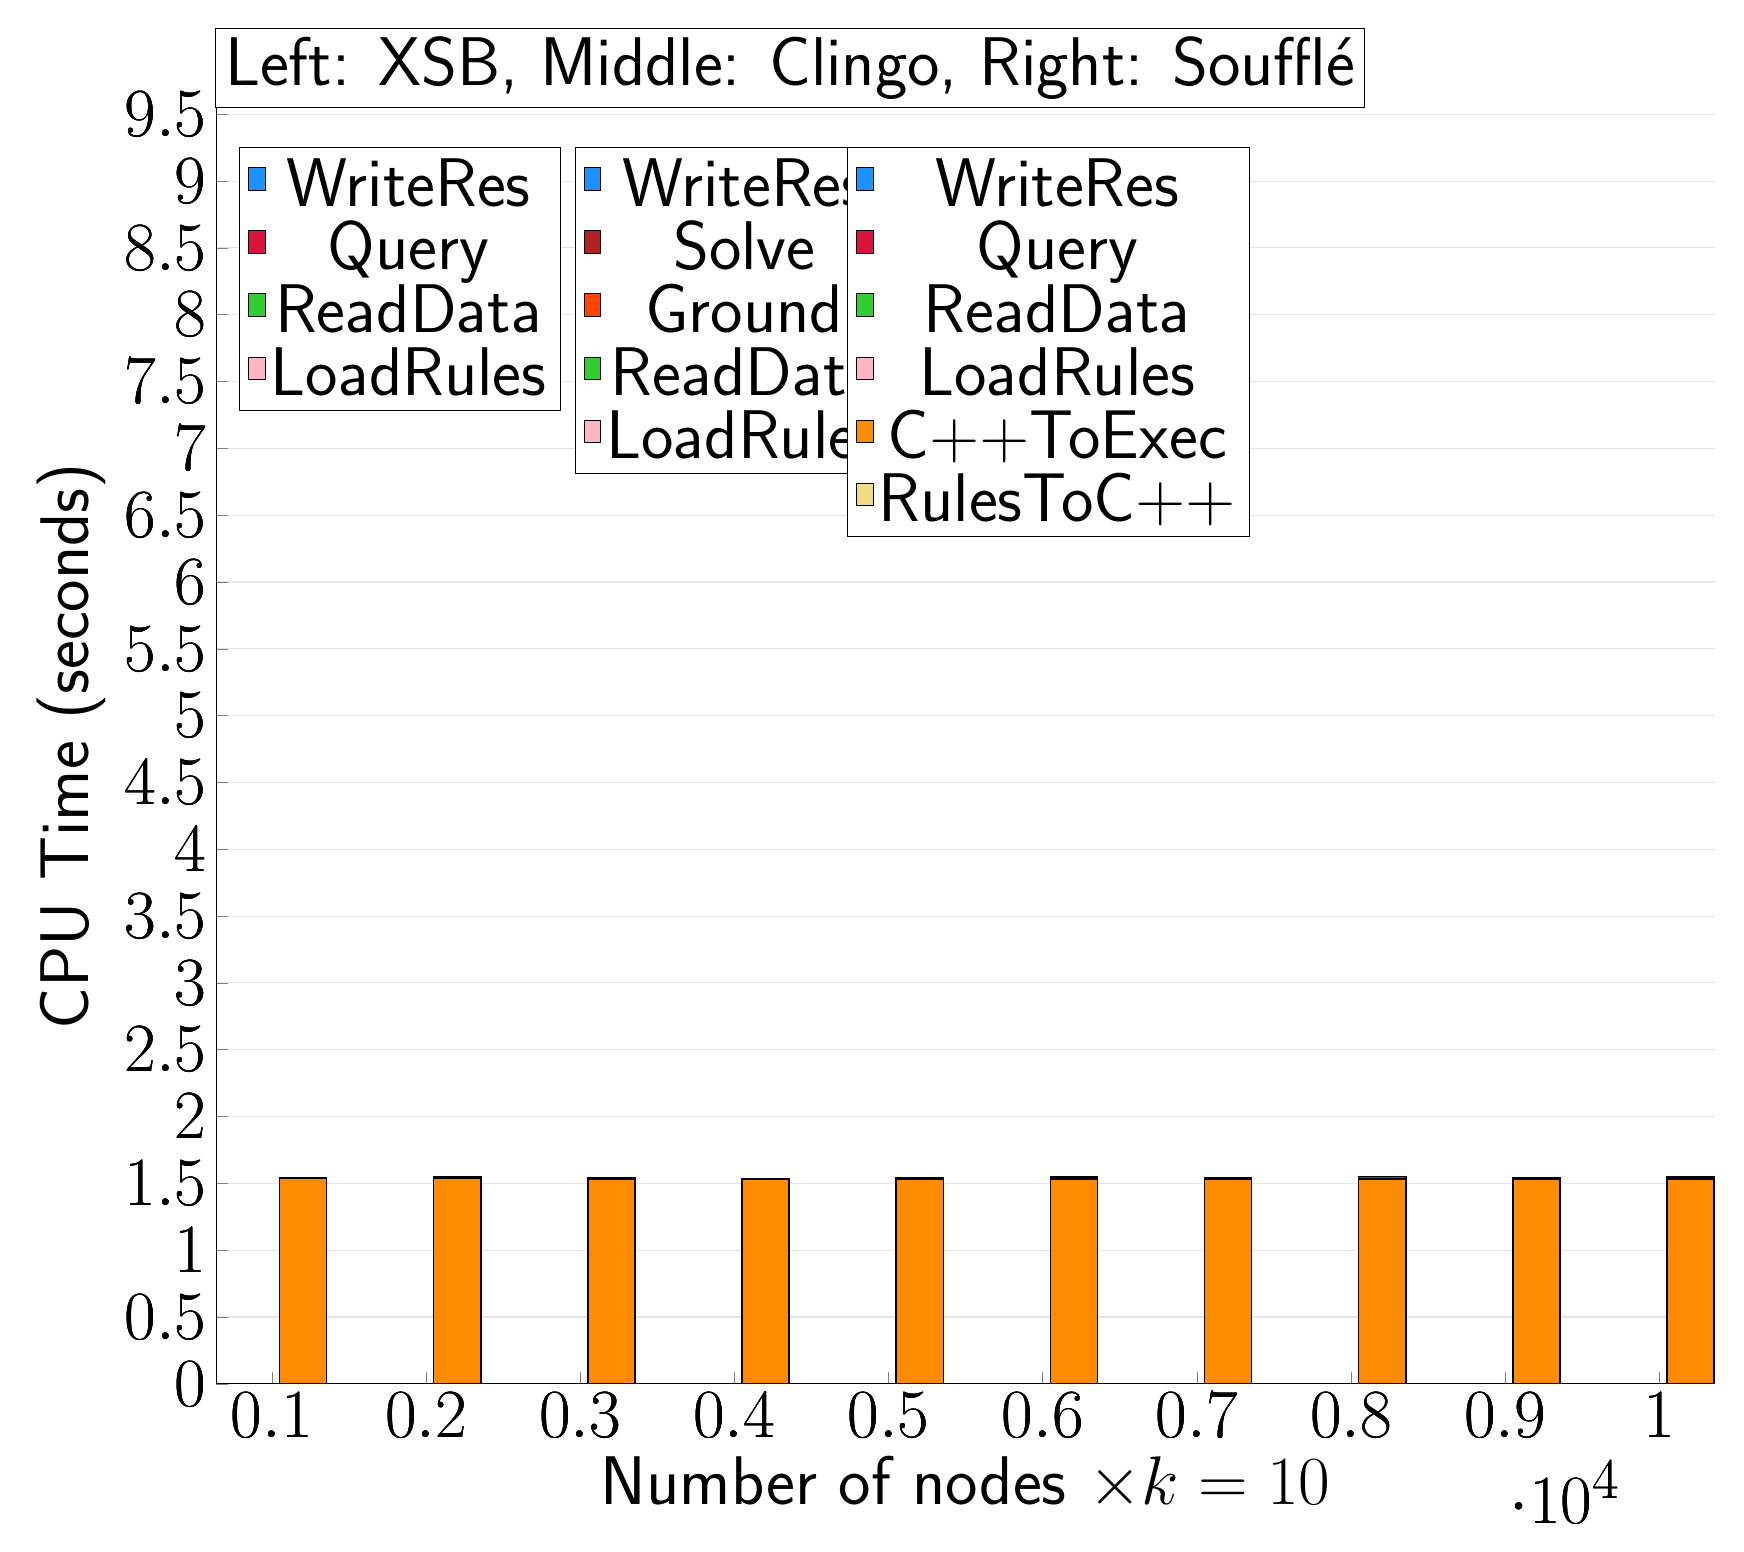
\begin{tikzpicture}
                        \begin{axis}[bar shift=-24.3pt, 
   ybar stacked,
   width=1.7\textwidth,
   bar width=0.6cm,
   ymajorgrids, tick align=inside,
   major grid style={draw=gray!20},
   xtick=data,
   ymin=0, ymax=9.544,
   axis x line*=bottom,
   axis y line*=left,
   enlarge x limits=0.04,
   legend style={
       at={(0.23, 0.97)},
       anchor=north east,
       legend columns=1,
       font=\Huge,
   },
   ylabel={CPU Time (seconds)},
   xlabel={Number of nodes $\times k=10$},
   label style={font=\Huge},
   tick label style={font=\Huge},
]
\addlegendimage{fill=DodgerBlue, draw=black, line width=0.2pt}
\addlegendentry{WriteRes}
\addlegendimage{fill=Crimson, draw=black, line width=0.2pt}
\addlegendentry{Query}
\addlegendimage{fill=LimeGreen, draw=black, line width=0.2pt}
\addlegendentry{ReadData}
\addlegendimage{fill=LightPink, draw=black, line width=0.2pt}
\addlegendentry{LoadRules}
\addplot +[fill=LightPink, draw=black, line width=0.55pt] coordinates {
(1000, 0.0005519999999999998)
(2000, 0.0005580000000000001)
(3000, 0.0005531999999999994)
(4000, 0.0005477999999999995)
(5000, 0.0005525999999999999)
(6000, 0.0005443999999999998)
(7000, 0.0005587999999999997)
(8000, 0.0005502)
(9000, 0.0005539999999999993)
(10000, 0.0005526000000000001)
};
\addplot +[fill=LimeGreen, draw=black, line width=0.55pt] coordinates {
(1000, 0.00020800000000000001)
(2000, 0.0002997999999999998)
(3000, 0.0003714000000000002)
(4000, 0.0004456)
(5000, 0.0005240000000000003)
(6000, 0.0006022)
(7000, 0.0006789999999999998)
(8000, 0.0007519999999999998)
(9000, 0.0008416000000000008)
(10000, 0.0009308000000000001)
};
\addplot +[fill=Crimson, draw=black, line width=0.55pt] coordinates {
(1000, 1.2599999999999781e-05)
(2000, 1.40000000000005e-05)
(3000, 1.320000000000004e-05)
(4000, 1.339999999999986e-05)
(5000, 1.219999999999974e-05)
(6000, 1.260000000000014e-05)
(7000, 1.2800000000000342e-05)
(8000, 1.3000000000000541e-05)
(9000, 1.239999999999958e-05)
(10000, 1.3399999999999878e-05)
};
\addplot +[fill=DodgerBlue, draw=black, line width=0.55pt] coordinates {
(1000, 6.440000000000056e-05)
(2000, 6.159999999999946e-05)
(3000, 6.35999999999994e-05)
(4000, 6.360000000000014e-05)
(5000, 6.480000000000022e-05)
(6000, 6.739999999999974e-05)
(7000, 6.479999999999922e-05)
(8000, 6.319999999999969e-05)
(9000, 6.380000000000098e-05)
(10000, 6.30000000000002e-05)
};
\end{axis}

\begin{axis}[bar shift=-6.5pt, 
   ybar stacked,
   width=1.7\textwidth,
   bar width=0.6cm,
   ymajorgrids, tick align=inside,
   major grid style={draw=none},
   xtick=data,
   ymin=0, ymax=9.544,
   axis x line*=none,
   axis y line*=none,
   enlarge x limits=0.04,
   legend style={
       at={(0.454, 0.97)},
       anchor=north east,
       legend columns=1,
       font=\Huge,
   },
   label style={font=\Huge},
   tick label style={font=\Huge},
]
\addlegendimage{fill=DodgerBlue, draw=black, line width=0.2pt}
\addlegendentry{WriteRes}
\addlegendimage{fill=FireBrick, draw=black, line width=0.2pt}
\addlegendentry{Solve}
\addlegendimage{fill=OrangeRed, draw=black, line width=0.2pt}
\addlegendentry{Ground}
\addlegendimage{fill=LimeGreen, draw=black, line width=0.2pt}
\addlegendentry{ReadData}
\addlegendimage{fill=LightPink, draw=black, line width=0.2pt}
\addlegendentry{LoadRules}
\addplot +[fill=LightPink, draw=black, line width=0.55pt] coordinates {
(1000, 0.0)
(2000, 0.0)
(3000, 0.0)
(4000, 0.0)
(5000, 0.0)
(6000, 0.0)
(7000, 0.0)
(8000, 0.0)
(9000, 0.0)
(10000, 0.0)
};
\addplot +[fill=LimeGreen, draw=black, line width=0.55pt] coordinates {
(1000, 0.0)
(2000, 0.0)
(3000, 0.0)
(4000, 0.0)
(5000, 0.0)
(6000, 0.0)
(7000, 0.0020000000000000018)
(8000, 0.0)
(9000, 0.0)
(10000, 0.0)
};
\addplot +[fill=OrangeRed, draw=black, line width=0.55pt] coordinates {
(1000, 0.0)
(2000, 0.0)
(3000, 0.0020000000000000018)
(4000, 0.0)
(5000, 0.0020000000000000018)
(6000, 0.0)
(7000, 0.0)
(8000, 0.0020000000000000018)
(9000, 0.0040000000000000036)
(10000, 0.0040000000000000036)
};
\addplot +[fill=FireBrick, draw=black, line width=0.55pt] coordinates {
(1000, 0.0)
(2000, 0.0)
(3000, 0.0)
(4000, 0.0)
(5000, 0.0)
(6000, 0.0)
(7000, 0.0)
(8000, 0.0)
(9000, 0.0)
(10000, 0.0)
};
\addplot +[fill=DodgerBlue, draw=black, line width=0.55pt] coordinates {
(1000, 0.0)
(2000, 0.0)
(3000, 0.0)
(4000, 0.0)
(5000, 0.0)
(6000, 0.0)
(7000, 0.0)
(8000, 0.0)
(9000, 0.0)
(10000, 0.0)
};
\end{axis}

\begin{axis}[bar shift=11.3pt, 
   ybar stacked,
   width=1.7\textwidth,
   bar width=0.6cm,
   ymajorgrids, tick align=inside,
   major grid style={draw=none},
   xtick=data,
   ymin=0, ymax=9.544,
   axis x line*=none,
   axis y line*=none,
   enlarge x limits=0.04,
   legend style={
       at={(0.69, 0.97)},
       anchor=north east,
       legend columns=1,
       font=\Huge,
   },
   label style={font=\Huge},
   tick label style={font=\Huge},
]
\addlegendimage{fill=DodgerBlue, draw=black, line width=0.2pt}
\addlegendentry{WriteRes}
\addlegendimage{fill=Crimson, draw=black, line width=0.2pt}
\addlegendentry{Query}
\addlegendimage{fill=LimeGreen, draw=black, line width=0.2pt}
\addlegendentry{ReadData}
\addlegendimage{fill=LightPink, draw=black, line width=0.2pt}
\addlegendentry{LoadRules}
\addlegendimage{fill=DarkOrange, draw=black, line width=0.2pt}
\addlegendentry{C++ToExec}
\addlegendimage{fill=LightGoldenrod, draw=black, line width=0.2pt}
\addlegendentry{RulesToC++}
\addplot +[fill=LightGoldenrod, draw=black, line width=0.55pt] coordinates {
(1000, 0.0020000000000000005)
(2000, 0.0)
(3000, 0.0)
(4000, 0.0)
(5000, 0.0)
(6000, 0.0)
(7000, 0.0)
(8000, 0.0)
(9000, 0.0)
(10000, 0.0)
};
\addplot +[fill=DarkOrange, draw=black, line width=0.55pt] coordinates {
(1000, 1.536)
(2000, 1.54)
(3000, 1.532)
(4000, 1.528)
(5000, 1.53)
(6000, 1.5340000000000003)
(7000, 1.53)
(8000, 1.5340000000000003)
(9000, 1.528)
(10000, 1.528)
};
\addplot +[fill=LightPink, draw=black, line width=0.55pt] coordinates {
(1000, 0.00015999999999999999)
(2000, 0.0001556)
(3000, 0.0001488)
(4000, 0.0001312)
(5000, 0.00015279999999999997)
(6000, 0.00014319999999999998)
(7000, 0.0001456)
(8000, 0.000147)
(9000, 0.00014739999999999998)
(10000, 0.00015240000000000002)
};
\addplot +[fill=LimeGreen, draw=black, line width=0.55pt] coordinates {
(1000, 0.0009368)
(2000, 0.0013936)
(3000, 0.0017065999999999997)
(4000, 0.0018308)
(5000, 0.002504)
(6000, 0.0027845999999999995)
(7000, 0.0031398000000000003)
(8000, 0.0035334)
(9000, 0.0037094000000000003)
(10000, 0.004148)
};
\addplot +[fill=Crimson, draw=black, line width=0.55pt] coordinates {
(1000, 0.0022492)
(2000, 0.0042412)
(3000, 0.005448800000000001)
(4000, 0.0068398)
(5000, 0.008859200000000001)
(6000, 0.0099412)
(7000, 0.0115032)
(8000, 0.0129388)
(9000, 0.0128408)
(10000, 0.0152)
};
\addplot +[fill=DodgerBlue, draw=black, line width=0.55pt] coordinates {
(1000, 0.0004476)
(2000, 0.00042040000000000003)
(3000, 0.00029939999999999996)
(4000, 0.0002934)
(5000, 0.0003036)
(6000, 0.0003086)
(7000, 0.00029639999999999994)
(8000, 0.0002722)
(9000, 0.0002626)
(10000, 0.0002648)
};
\end{axis}


\node[anchor=south, draw, fill=white] at (rel axis cs:0.42,1) {\Huge Left: XSB, Middle: Clingo, Right: Soufflé};
\end{tikzpicture}
\end{document}
                    